\section{第~\ref{sec:one-shot}~节的详细信息}

\subsection{实验设置与训练查询}
\label{app:model-data}

\paragraph{遵循指令的设置。}
\label{app:IF-setup}
与其他主领域教师不同，指令遵循教师模型是专门为我们的实验训练的。我们从 DeepSeek-R1-Distill-Qwen-1.5B 出发，在具有可编程验证约束的合成指令遵循任务上对该模型进行后训练。我们采用 GRPO 方法，并使用基于规则的结果奖励，以指示响应是否满足目标轮次约束。训练时每个提示生成四个补全，温度设为 \(0.9\)；最大提示长度为 \(4{,}096\) 个 token，最大响应长度为 \(16{,}384\) 个 token；优化器采用 AdamW，学习率为 \(1\times10^{-6}\)，训练批量大小为 \(16\)，裁剪比为 \(0.2\)。第 600 步的检查点被用作指令遵循教师模型，使 IFBench \citep{pyatkin2026generalizing} 从 \(14.33\) 提升至 \(20.65\)，Multi-IF 最终轮次准确率从 \(20.84\) 提升至 \(28.58\)。

对于该领域，“full-data”表示从 UltraData-SFT-2605 \citep{ultradata-sft-2605} 中采样的子集，而非完整数据集，且 one-shot 查询随机从中选取。


\paragraph{针对 one-shot OPD 的数学查询（表~\ref{tab:one-shot-queries}，图~\ref{fig:probe_prompt_training_acc}）。}
\label{app:training-accuracy}
我们从未经训练的学生模型中为 DAPO-Math-17K 的前 64 个查询中的每一个采样 8 次轨迹，并根据最终通过率分配难度，从而选定 \texttt{t59} (\(8/8\) )、\texttt{t22} (\(4/8\) ) 和 \texttt{t56} (\(0/8\) ) 分别作为简单、中等和困难的查询。在训练过程中，每个查询被解决的频率符合这一分配：简单查询始终维持在 \(1.0\) 左右，中等查询从 \(0.36\) 上升至约 \(0.89\) ，而困难查询在 \(300\) 步内从未被解决，然而如图~\ref{fig:probe_prompt} 所示，这三个查询均带来了相近的基准提升。

\begin{table}[t]
    \centering
    \small
    \setlength{\tabcolsep}{4pt}
    \begin{tabular}{p{0.10\textwidth}p{0.08\textwidth}p{0.74\textwidth}}
    \toprule
    Difficulty & ID & Query \\
    \midrule
    Easy & \texttt{t59} &
    In triangle \(ABC\), let \(D\) be the foot of the altitude from \(A\). Suppose that \(AD=4\), \(BD=3\), \(CD=2\), and \(AB\) is extended past \(B\) to a point \(E\) such that \(BE=5\). Determine the value of \(CE^2\). \\
    \midrule
    Medium & \texttt{t22} &
    Let \(S\) be the set of triples \((a,b,c)\) of non-negative integers such that \(a+b+c\) is even. Determine the value of
    \(\sum_{(a,b,c)\in S} \frac{1}{2^a3^b5^c}\).
    This sum can be expressed as \(\frac{m}{n}\), where \(m\) and \(n\) are relatively prime positive integers. Compute \(m+n\). \\
    \midrule
    Hard & \texttt{t56} &
    Byan is playing a game called ``raven, raven, falcon'' with his three friends. His friends sit in a circle, and Byan walks clockwise around them, tapping each friend he passes on the head and saying either ``raven'' or ``falcon,'' each with probability \(\frac{1}{2}\). The game ends when Byan has said ``falcon'' twice. The probability that one of his friends will be called a ``falcon'' twice can be expressed as \(\frac{m}{n}\), where \(m\) and \(n\) are relatively prime positive integers. Find \(100m+n\). \\
    \bottomrule
    \end{tabular}
    \caption{在查询难度实验中使用的数学查询，按学生在OPD训练前的通过率进行标签标注。}
    \label{tab:one-shot-queries}
\end{table}

\begin{figure}[t]
    \centering
    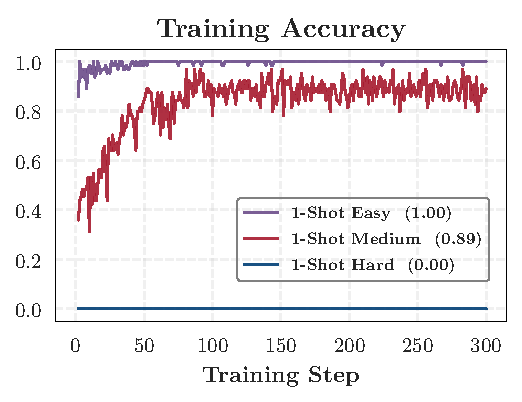
\includegraphics[width=0.45\linewidth]{figures/3A_ablations_training_acc.pdf}
    \caption{每个步骤中，64次滚动采样中有多少比例能够解决训练查询本身，针对表~\ref{tab:one-shot-queries}中的三个查询。}
    \label{fig:probe_prompt_training_acc}
\end{figure}

\paragraph{OPD 的默认超参数（表~\ref{tab:opd-hyperparams}）。}
除非另有说明，所有实验均使用以下默认设置。top-\(K\) 行涵盖了两个目标：第~\ref{sec:finding-recovery}~节中的数学 one-shot 运行使用 \(K=16\) ，而所有其他实验均使用采样 token 目标。

\begin{table}[t]
\centering
\caption{OPD的默认超参数。}
\label{tab:opd-hyperparams}
\small
\begin{tabular}{ll}
\toprule
\textbf{Item} & \textbf{Value} \\
\midrule
Rollout batch size      & 64 \\
Mini batch size         & 64 \\
Responses per prompt    & 1 \\
KL coefficient          & 0.0 \\
LogProb top-$K$         & 0(default) / 16 \\
Top-$K$ strategy        & Student Top-$K$ \\
Loss aggregation        & token-mean \\
Training temperature    & 1.0 \\
Top-$p$                 & 1.0 \\
Optimizer               & AdamW ($\beta_1{=}0.9$, $\beta_2{=}0.999$, wd $=0.01$) \\
Learning rate           & 1e-6 \\
Gradient clip norm      & 1.0 \\
Max prompt length       & 1024 (math); 4096 (code, IF, agentic) \\
Max response length     & 7168 (math, code, IF); 2048 (agentic) \\
\bottomrule
\end{tabular}
\end{table}


\section{第~\ref{sec:data}~节的详细信息}

\subsection{训练状态覆盖}
\label{app:state-coverage}
\label{app:state-coverage-robustness}

\paragraph{建设。}
每个优化步骤收集轨迹而非随机收集，以确保训练的每个阶段都得到同等表示，且各情景下的预算具有可比性，这些情景均运行相同步数：在完整数据运行的从 \(1\) 到 \(500\) 每一步中，我们获取 \(5\) 条轨迹，其中三条用于构建簇，两条构成完整数据（保留）部分，共 \(12{,}000\) 条参考状态和 \(8{,}000\) 条保留状态。通过PAC将这些轨迹降维至 \(50\) 维，保留 \(71.9\%\) 的方差，再进行 \(K\) -均值聚类。随后，对每个评估情景均按相同调度进行测量，在每一步抽取 \(2\) 条来自 \(5\) 条轨迹的样本，并在整个训练过程中累积，使得第 \(300\) 步的预算 \(600\) 条轨迹与保留分割相匹配。该抽样过程重复 \(30\) 次；带状区域和误差条表示这些重复结果的标准差，反映了轨迹下采样带来的差异，而非不同训练模型之间的变化。

\paragraph{该排序在 \(K\) 、参考构建以及状态位置上均保持稳定（表~\ref{tab:coverage-k} 和~\ref{tab:coverage-reference}，图~\ref{fig:state-position-sensitivity}）。}
覆盖度取决于参考状态的聚类精细程度以及定义簇的状态，因此我们同时改变这两个因素。第一张表重复了分析，\(K\in\{50,100,200,500\}\) 时更细的簇导致绝对覆盖度降低，但覆盖度仍从1-shot到4-shot再到16-shot逐步提升，16-shot接近全数据情况。第二张表则基于每个情景下\(2{,}000\) 次滚动结果的并集重建簇，而非仅基于全数据状态，其排序依然成立；由于来自所有情景的状态共同定义了这些合并簇，合并覆盖度并非恢复度量，其各行仅应相互比较。图中改变了从每次滚动读取的位置，将最终非填充token与固定绝对位置\(2{,}000\) 和\(4{,}000\) 与主分析中的8个相对位置进行对比。四种情况均保持了相同排序。固定位置变体的结果接近主构造，而最终token在查询较少时给出显著更低的覆盖度，这正是由响应长度和终止决定位置所预期的结果；因此我们采用8个相对位置，可对任意长度的响应进行全程采样。

\begin{table}[t]
    \centering
    \small
    \caption{全数据锚定训练状态覆盖，步骤 \(300\)  下不同簇数量 \(K\)  时。}
    \label{tab:coverage-k}
    \begin{tabular}{lcccc}
        \toprule
        \(K\)
        & 1-shot
        & 4-shot
        & 16-shot
        & Full data (held-out) \\
        \midrule
        50  & 0.755 & 0.829 & 1.000 & 1.000 \\
        100 & 0.727 & 0.803 & 1.000 & 1.000 \\
        200 & 0.715 & 0.798 & 0.989 & 1.000 \\
        500 & 0.564 & 0.695 & 0.904 & 0.956 \\
        \bottomrule
    \end{tabular}
\end{table}

\begin{table}[t]
    \centering
    \small
    \caption{在不同簇构造下的训练状态覆盖，当 \(K=200\) 时。}
    \label{tab:coverage-reference}
    \begin{tabular}{lcccc}
        \toprule
        Reference construction
        & 1-shot
        & 4-shot
        & 16-shot
        & Full data (held-out) \\
        \midrule
        Full-data anchored
        & 0.663 & 0.773 & 0.953 & 0.998 \\
        Equal-size pooled
        & 0.750 & 0.845 & 0.958 & 0.966 \\
        \bottomrule
    \end{tabular}
\end{table}

\begin{figure}[t]
    \centering
    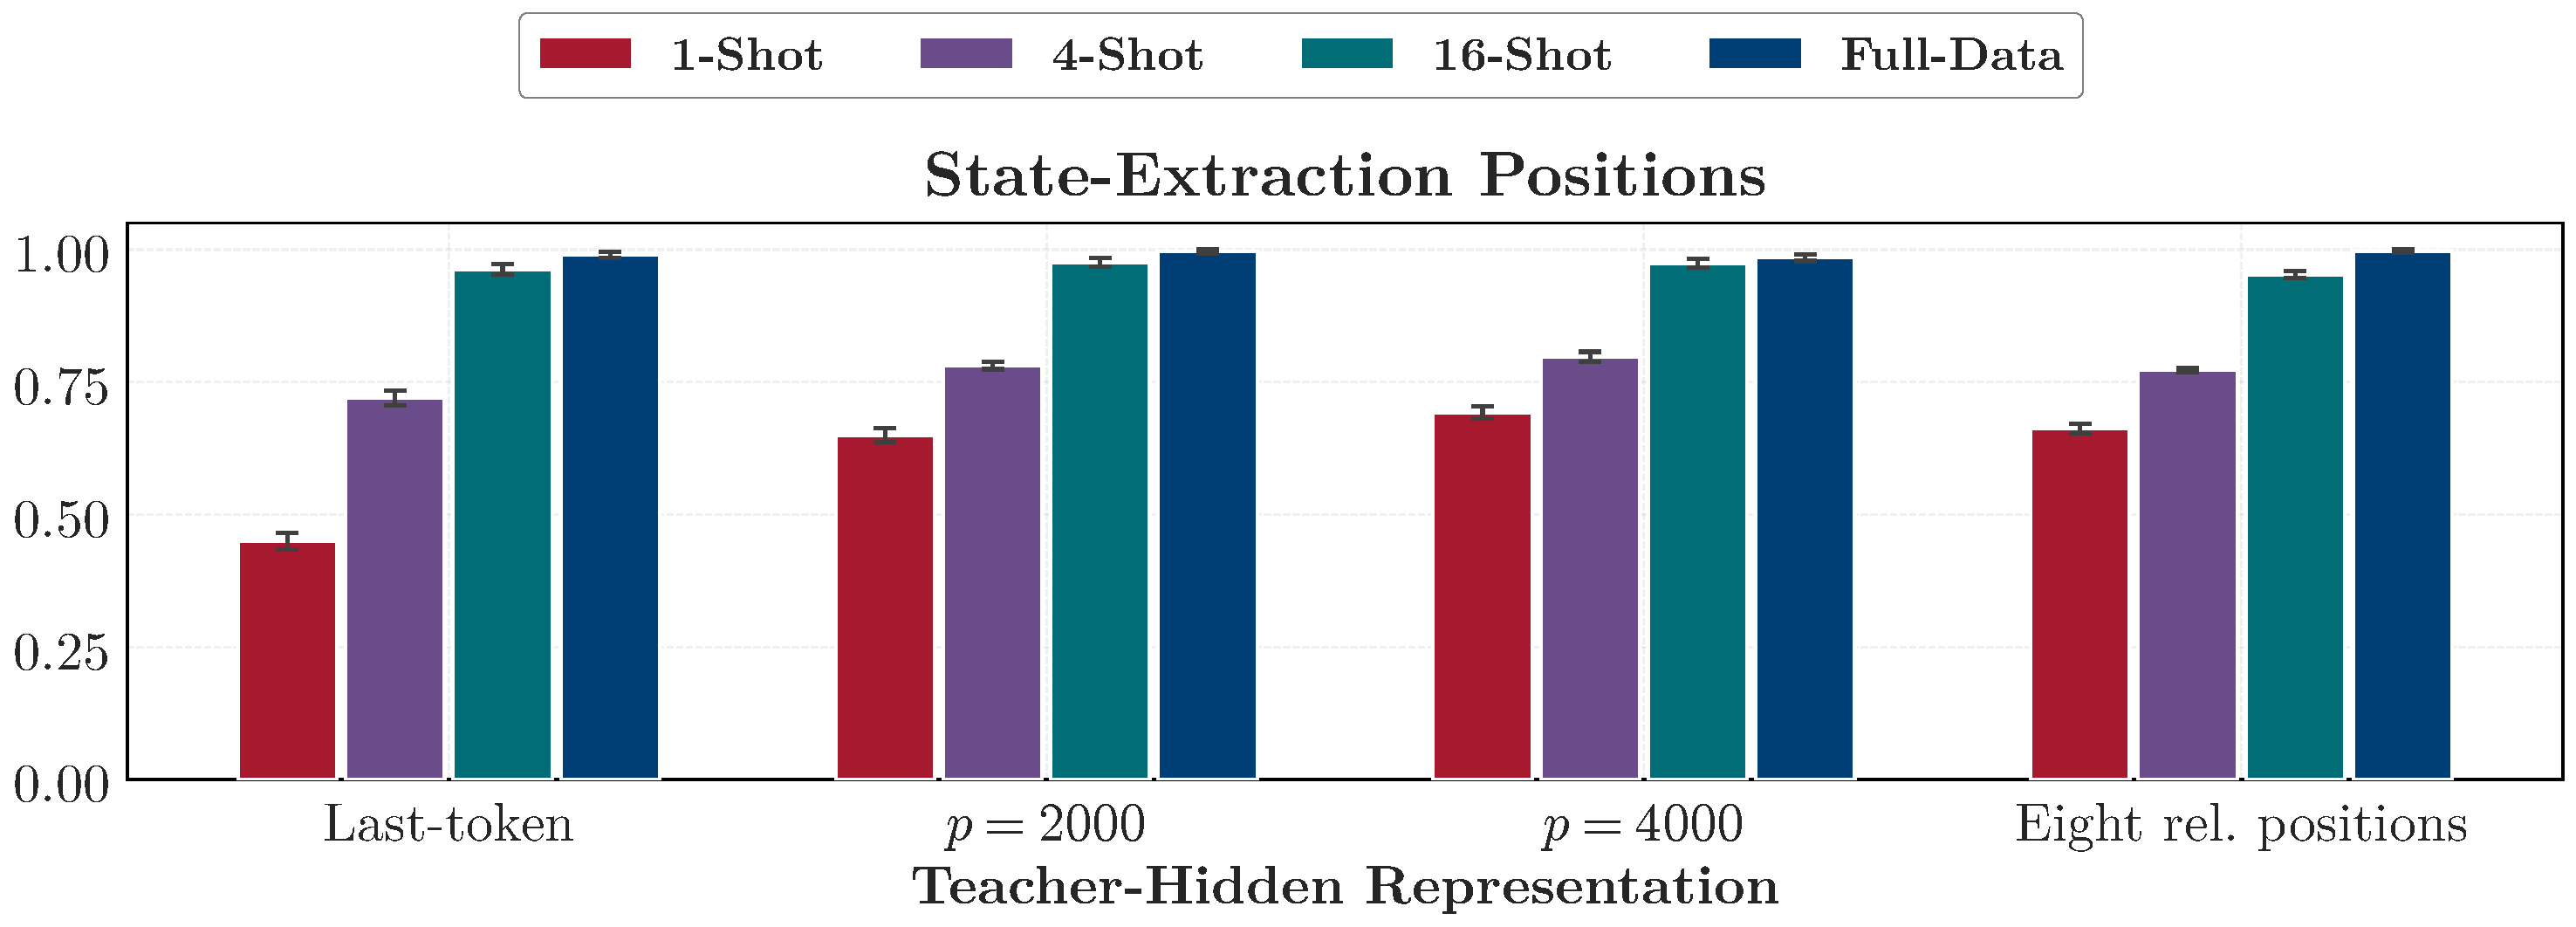
\includegraphics[width=0.85\linewidth]{figures/4A_state_extraction_positions.pdf}
    \caption{在不同状态提取位置下的训练状态覆盖，对应 \(K=200\)。误差条表示滚动子采样的一标准差。}
    \label{fig:state-position-sensitivity}
\end{figure}

\paragraph{one-shot 具有更重的远距离状态尾部，但与完整数据不可分离（表~\ref{tab:reference-diagnostics}）。}
最近质心分配将一个状态分配到某个簇中，即使它与所有全数据状态的距离都很远，因此仅靠覆盖无法区分参考空间填充稀疏的情景与填充较密的情景。因此，我们还测量每个状态在未缩减的 \(1536\) 维空间中与其十个最近参考状态的平均余弦距离，并在该距离超过保留样本中全数据状态的 \(95\) 百分位数时，将该状态标记为非参考状态。one-shot OPD 超过阈值的频率高于其他情景，因此其距离分布的上尾更重。然而，与保留的全数据状态相比，其 AUROC 为 \(0.552\)，接近随机水平，说明 one-shot 状态整体上不可分离于全数据状态。

\begin{table}[t]
    \centering
    \small
    \caption{不同查询集大小下的参考距离诊断。AUROC 将每个情景与保留的完整数据状态进行比较。最后一行是包含构建簇所用回放数据的完整数据池，因此其超过率无需等于 \(5\%\)  所设定的阈值。}
    \label{tab:reference-diagnostics}
    \begin{tabular}{lccc}
        \toprule
        Setting
        & Exceedance (\%)
        & Mean distance
        & AUROC \\
        \midrule
        1-shot   & 17.2 & 0.283 & 0.552 \\
        4-shot   & 4.4  & 0.218 & 0.477 \\
        16-shot  & 3.8  & 0.231 & 0.512 \\
        Full data (all)  & 4.0  & 0.215 & 0.476 \\
        \bottomrule
    \end{tabular}
\end{table}

\subsection{训练数据的控制}
\label{app:fixed-count-diversity}
\label{app:schedule}

\paragraph{16-shot OPD 中的多样性（图~\ref{fig:fixed-count-diversity}）。}
阶梯中第~\ref{sec:state-diversity}~节的每个查询代表一个不同的语义簇，因此同时提升了多样性和数量。保持数量为16，并从单一簇中抽取第二组数据进行分离：这16个簇代表在步骤~\(300\)~处达到~\(70.9\)~的有效准确率，而单一簇组仅为~\(69.9\)~，这大约相当于4次采样OPD使用四分之一查询量所达到的水平，其状态覆盖也以相同方式分离，并且更早实现，~\(98.9\%\)~，而单一簇组在~\(76.8\%\)~附近趋于平坦，仅在~\(100\)~步内完成。来自单一簇的查询会不断将学生带回其已访问过的状态空间部分。

\begin{figure}[t]
  \centering
  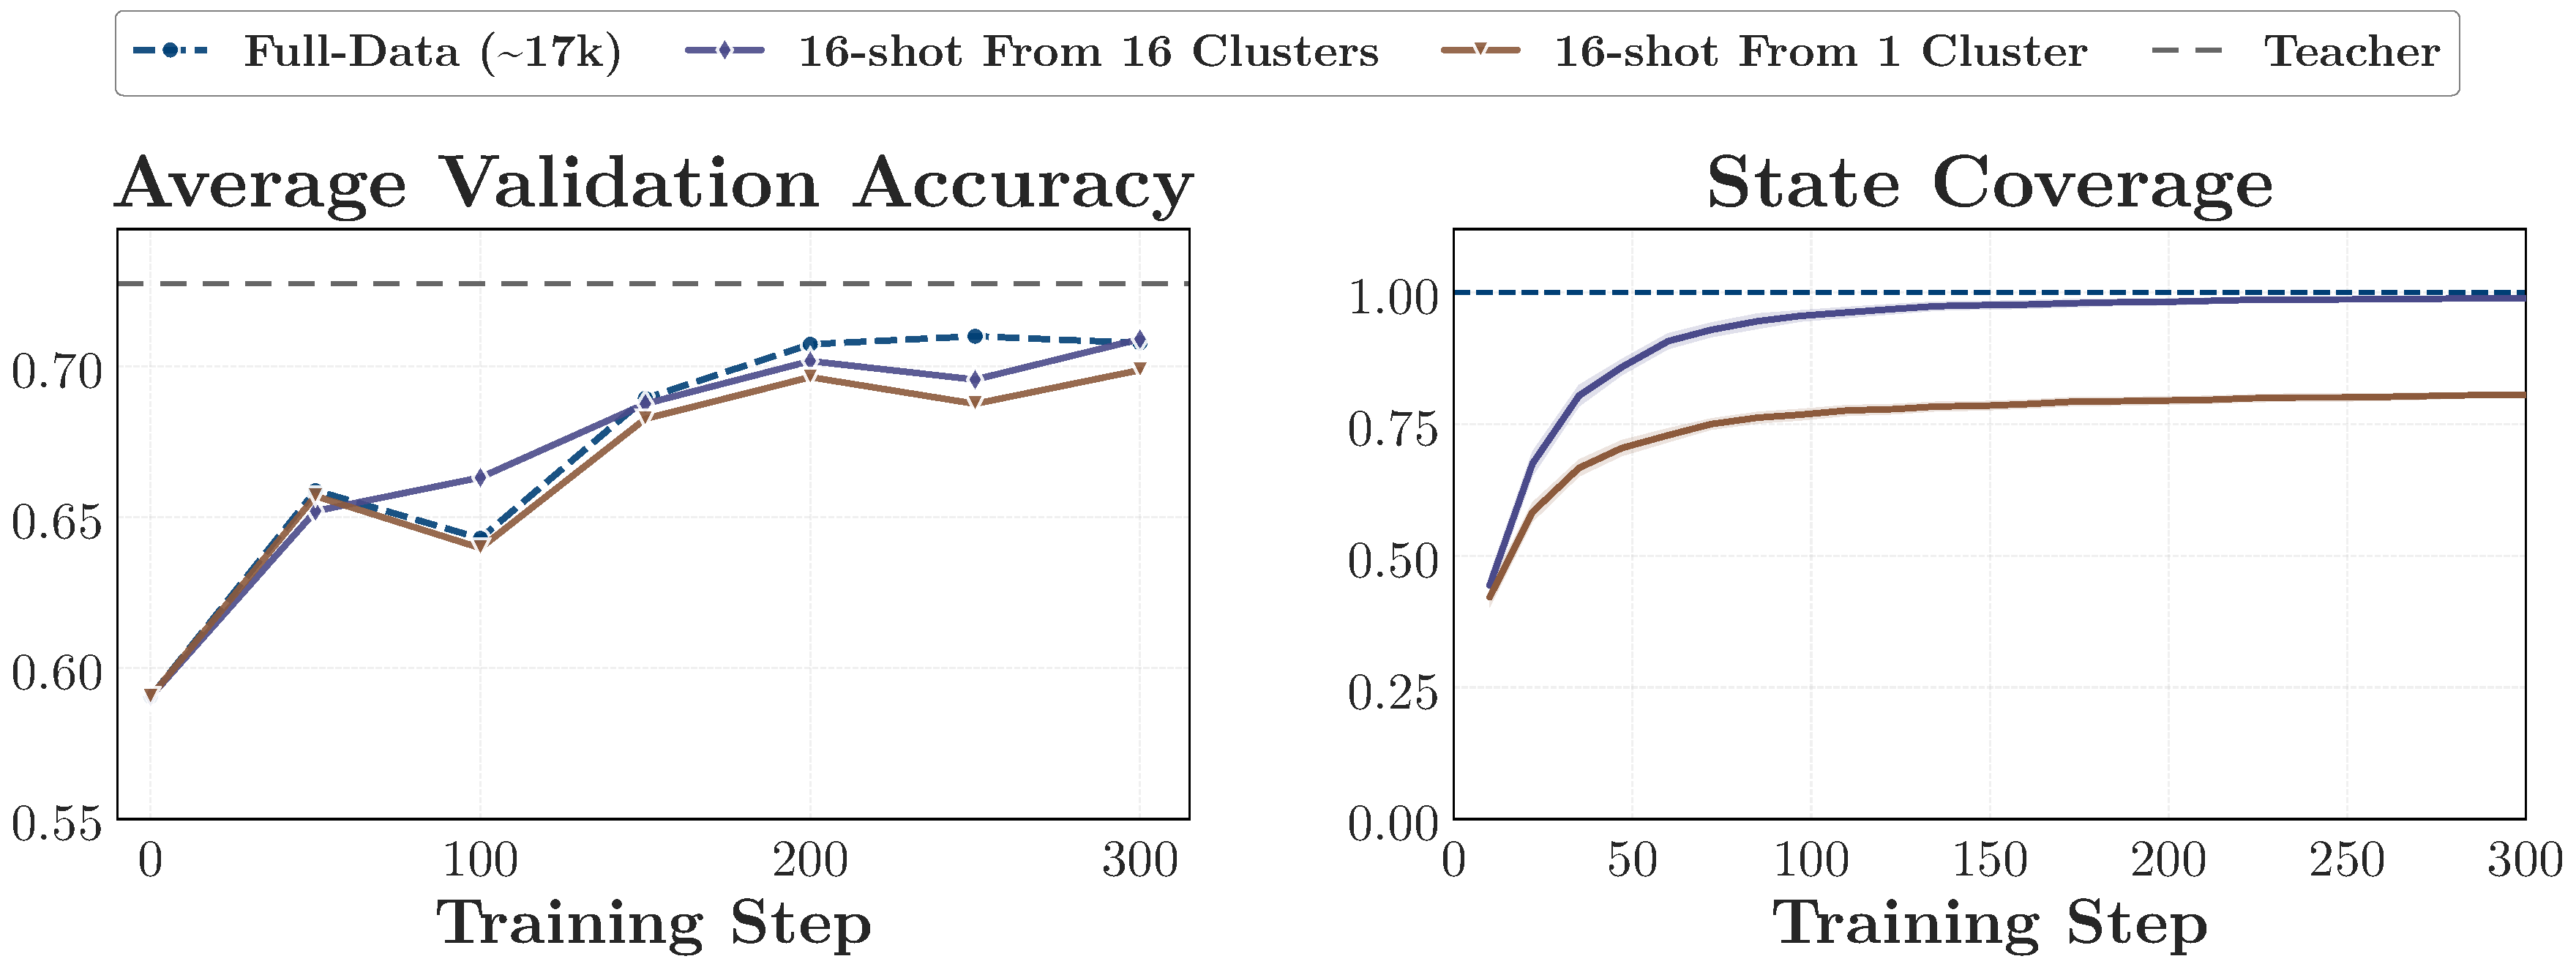
\includegraphics[width=0.75\linewidth]{figures/4A_nshot_diversity.pdf}
  \caption{两个仅在多样性上不同的16次查询集，与全数据OPD进行对比。}
  \label{fig:fixed-count-diversity}
\end{figure}

\paragraph{在 2 次查询 OPD（图~\ref{fig:nshot_schedule}）中的查询调度。}
固定一个双查询集，仅改变每个查询的呈现时机：顺序调度在 \(600\) 步预算的前 \(300\) 步上训练困难查询，剩余步数则训练中等难度查询；而混合调度则在每个批量中各放入 \(32\) 份困难查询和中等难度查询。在第 \(600\) 步时，二者分别达到 \(68.8\) 和 \(69.1\) ，均高于它们共享的 one-shot 基准的 \(67.4\) ，因此，在第二个查询本身所带来的收益面前，对固定查询集进行排序几乎无关紧要。这些实验的训练时长远超第~\ref{sec:state-diversity} 节中的实验，并以困难查询作为其基准，故其时间范围（horizon）与基准均不可与图~\ref{fig:state-diversity} 中的结果互换。

\begin{figure}[t]
  \centering
  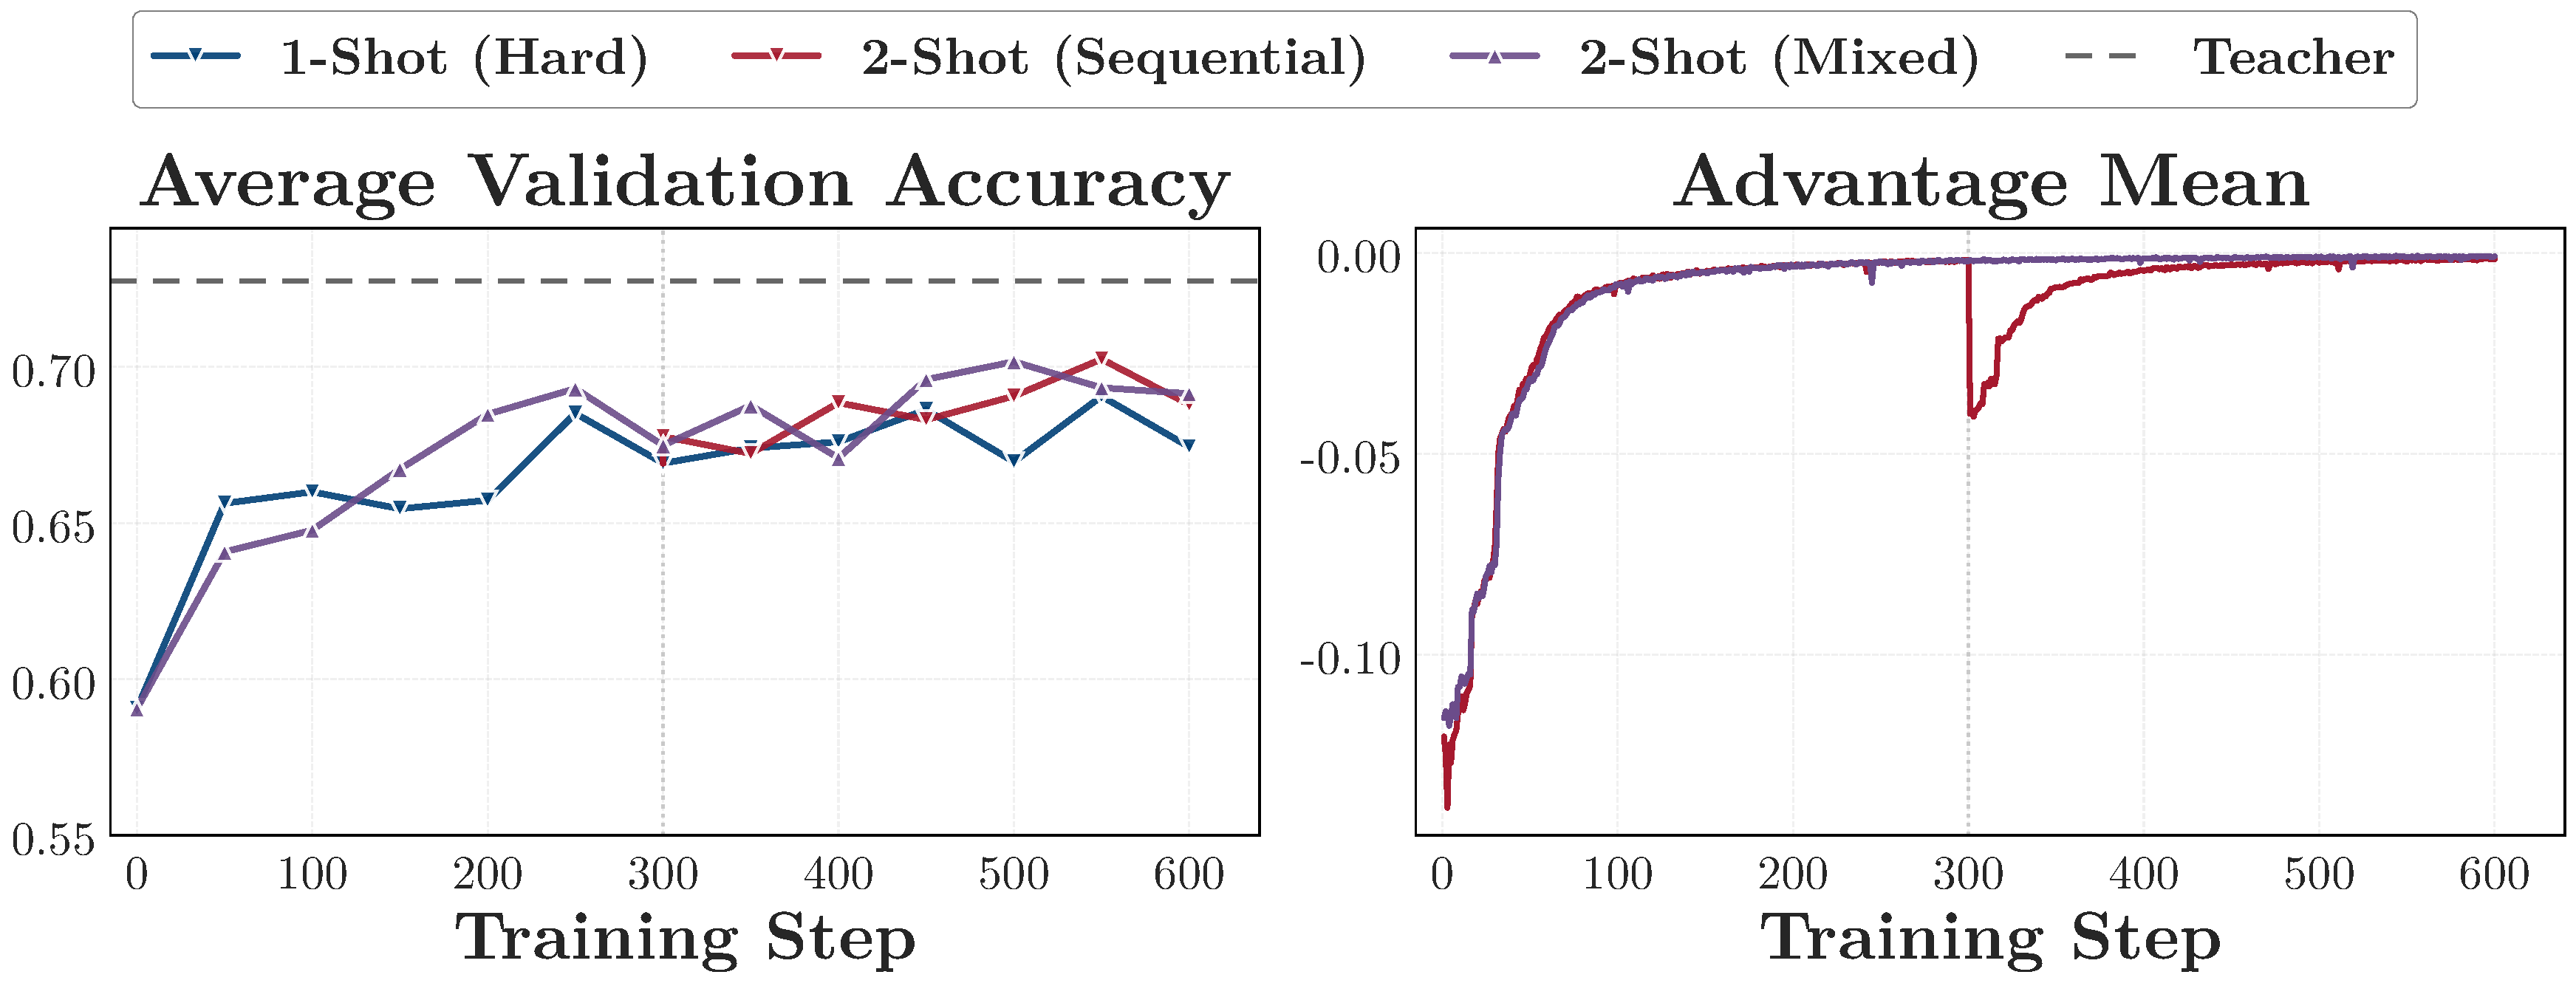
\includegraphics[width=0.75\linewidth]{figures/4A_2shot_schedule.pdf}
  \caption{2-shot OPD中查询调度的影响。垂直虚线标记了顺序调度中的查询切换点。}
  \label{fig:nshot_schedule}
\end{figure}

\section{第~\ref{sec:algorithm}~节的详细信息}

\subsection{估算吸收率和测量窗口}
\label{app:alignment-dynamics}

第~\ref{sec:mech-dynamics} 节在三种不同约定下进行测量。为何每一种：
\begin{itemize}[topsep=2pt, partopsep=0pt, leftmargin=13pt, itemsep=2pt, parsep=0pt]
    \item  \(\boldsymbol{[t/1.4,\,1.4t]}\) . 当 \(d\)  缓慢移动时，相邻步长之间的差异主要为噪声，因此 \(v_t\)  被视为该窗口两端点间 \(\log d\)  的斜率，使用每个端点附近的中位数 \(d\)  进行计算。仅当窗口完全位于测量值域内的中心点才会被绘制，这也是主文中读取步骤 \(50\)  和 \(200\)  的速率，而非步骤 \(300\)  的原因。
    \item  \(\boldsymbol{d_t/d_{30}}\)。每次运行测量其访问状态的距离，四个在每一步上处于不同层级 \(30\)，因此将其各自值绘制在对应位置，可使曲线通过形状而非层级进行比较。
    \item  \textbf{从步骤 \(30\) 开始。} 梯度裁剪在此前一直有效，而裁剪后的更新并非目标所要求的更新：\(v_t\) 在该窗口内衡量的是一个\emph{固定大小}步长所带来的收益，而非一个步长所带来的收益，这就是为什么在该处测量到的速率上升而非下降的原因。
\end{itemize}

表~\ref{tab:gap-reduction} 汇总了第~\ref{sec:mech-dynamics} 节引用的该值域中的数据：在步骤 \(300\) 时，步长-\(30\) 距离剩余的比例，以及步骤 \(50\) 与 \(200\) 之间吸收率下降的因子。

\begin{table}[t]
    \centering
    \small
    \caption{同策略 OPD 在默认学习率下的步数对齐动态 \(30\) --\(300\)。}
    \label{tab:gap-reduction}
    \begin{tabular}{lcccc}
        \toprule
        Setting (queries) & 1 & 4 & 16 & Full data \\
        \midrule
        \(d_{300}/d_{30}\) & 0.16 & 0.17 & 0.18 & 0.22 \\
        \(v_{50}/v_{200}\) & 5.6 & 5.2 & 4.2 & 6.4 \\
        \bottomrule
    \end{tabular}
\end{table}

\subsection{学习率重新缩放了步长轴}
\label{app:lr-sensitivity}

我们重复同策略 one-shot OPD，分别在半倍、默认以及两倍于默认学习率的情景下进行，保持其他所有设置不变，并在同一 \(300\) 步数范围内读取全部三种情况的结果，如第~\ref{sec:mech-dynamics} 节所述。

\begin{figure}[t]
    \centering
    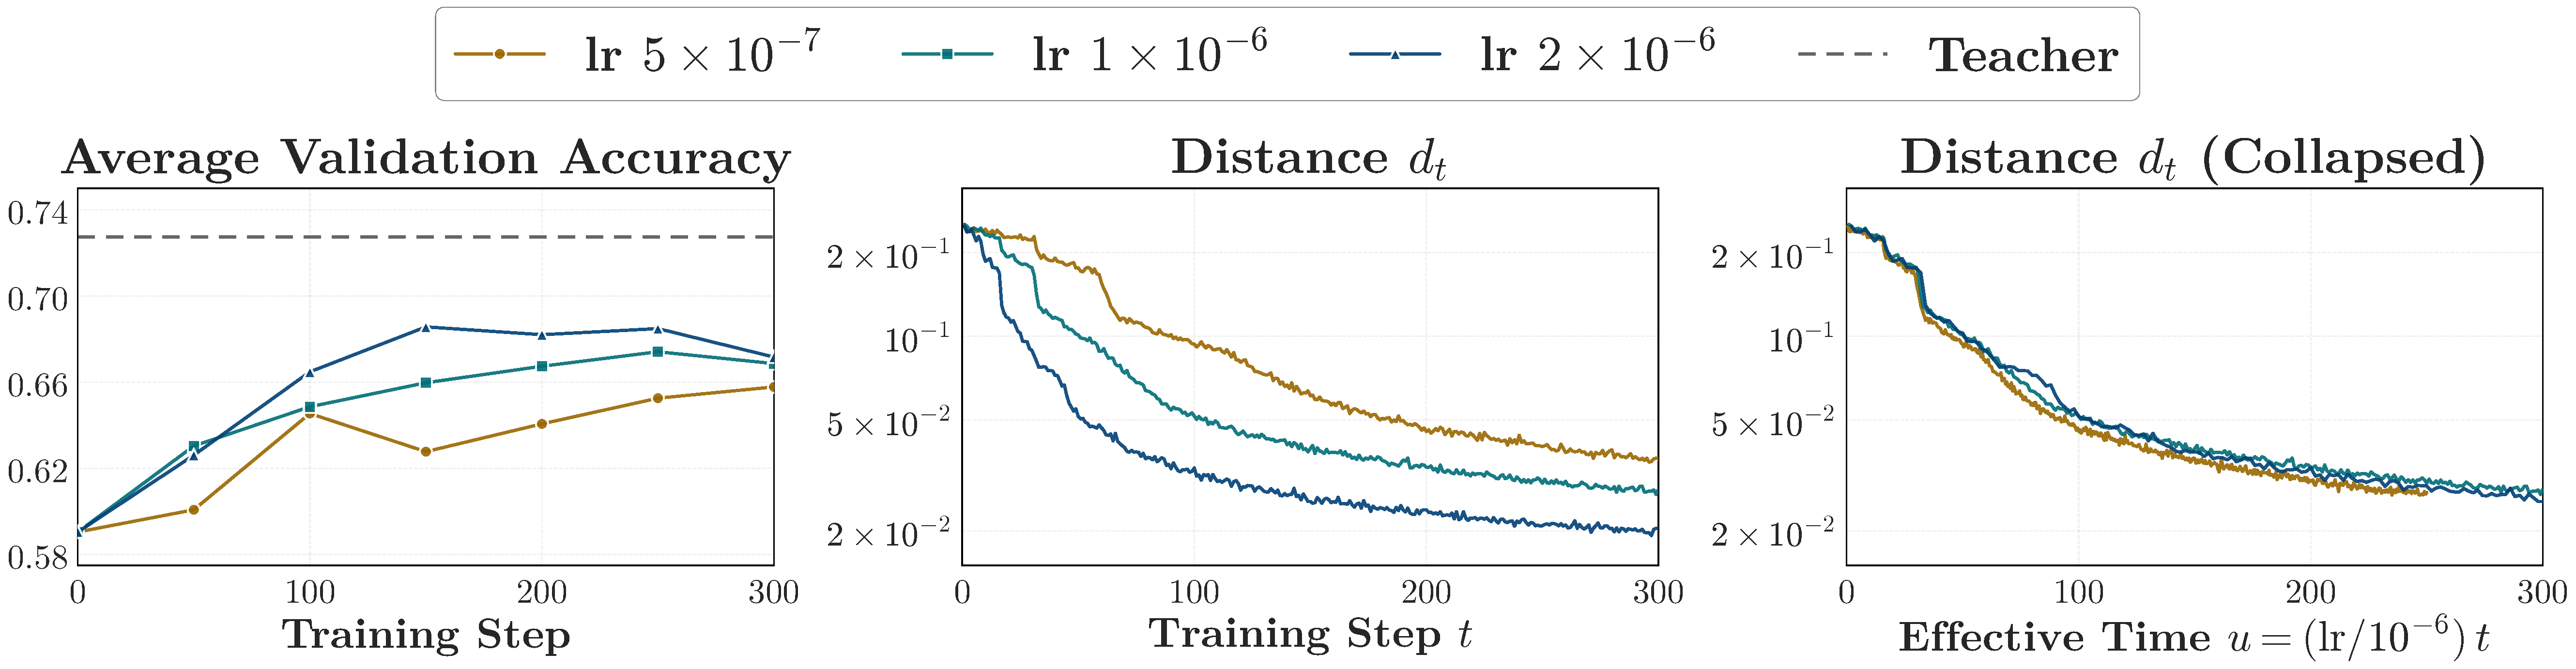
\includegraphics[width=\linewidth]{figures/5A_lr_collapse_v2.pdf}
    \caption{one-shot OPD 在一半、正常和两倍默认学习率下的验证准确率与教师-学生距离。距离以对数刻度的纵轴表示，时间以线性刻度表示。}
    \label{fig:lr-sensitivity}
\end{figure}

\paragraph{学习率会缩放步长轴，而保持减速部分不变。}
较大的学习率会更早达到任意给定的距离，三条曲线之间的分离程度大致与学习率的比值成比例（图~\ref{fig:lr-sensitivity}）。将横轴从步数 \(t\) 改为 \(u=(\mathrm{lr}/10^{-6})\,t\) 后，它们便重合为一条曲线：三次运行之间的差距从约 \(2.2\times\) 缩小到约 \(1.1\times\)。因此，学习率仅决定了运行沿该曲线移动的速度，而不会改变曲线本身的形状。随着距离增加，曲线变得越来越平坦，正如第~\ref{sec:mech-dynamics} 节中四种查询情景相对于步数的表现一样。因此，在我们测试的四倍范围中，成比例更大的学习率会成比例地缩短运行时间，而不会触及导致对齐变慢的初始原因。


\section{第~\ref{sec:mopd}~节的详细信息}
表~\ref{tab:mopd-hyperparams} 显示了MOPD的默认超参数。

\begin{table}[!ht]
\centering
\caption{MOPD（多教师同策略蒸馏）的默认超参数。}
\label{tab:mopd-hyperparams}
\small
\begin{tabular}{ll}
\toprule
\textbf{Item} & \textbf{Value} \\
\midrule
Number of teachers      & 3 (math / code / IF) \\
LogProb top-$k$         & 0  \\
KL coefficient          & 0.0 \\
Loss aggregation        & seq-mean-token-mean \\
\midrule
Rollout batch size      & 64 \\
Mini batch size         & 64 \\
Responses per prompt    & 1 \\
Training temperature    & 1.0 \\
Top-$p$                 & 1.0 \\
\midrule
Optimizer               & AdamW ($\beta_1{=}0.9$, $\beta_2{=}0.999$, wd $=0.01$) \\
Learning rate           & 1e-6 \\
Gradient clipping       & 1.0 \\
\midrule
Max prompt length       & 4096 \\
Max response length     & 7680 \\
\bottomrule
\end{tabular}
\end{table}


\section{第~\ref{sec:discussion}~节的详细信息}

\subsection{代码生成中的模板与WildChat OPD}
\label{app:template-code}

第~\ref{sec:template} 节报告了数学中的四种输入条件。此处我们报告代码生成中的相同四种条件。

\paragraph{设置}
该学生模型为 R1-Distill-1.5B，教师模型为 DeepCoder-1.5B-Preview~\citep{deepcoder2025}，基准模型为 TACO~\citep{li2023taco} 上的全数据 OPD。基础模板、系统模板和 WildChat 查询与第~\ref{sec:template} 节中的完全一致；系统模板中的一行指令为图~\ref{fig:template-examples}b 中的竞赛编程指令。我们在 LiveCodeBench v6 上以 avg@3 为评估指标进行评测。

\begin{figure}[!htb]
  \centering
  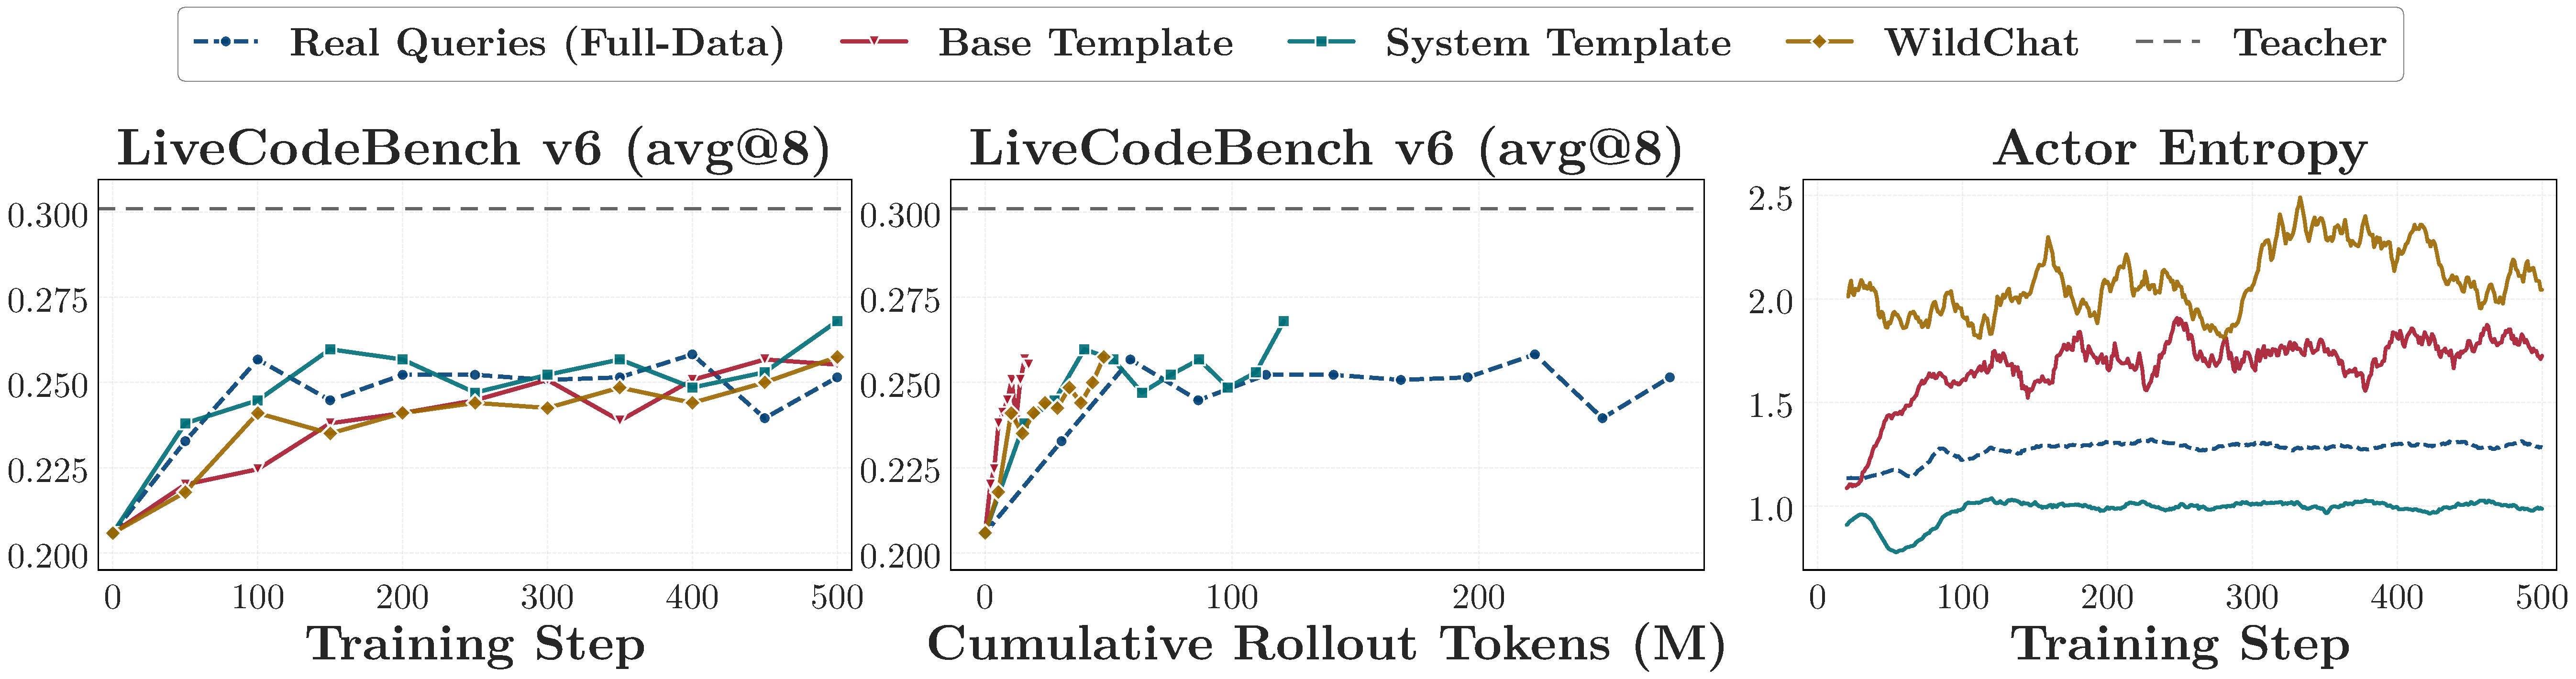
\includegraphics[width=\textwidth]{figures/7A_template_wildchat_code.pdf}
  \caption{代码生成OPD的验证准确率和演员熵。
  }
  \label{fig:template-wildchat-code}
\end{figure}

\paragraph{结果。}
图~\ref{fig:template-wildchat-code} 显示了四种情况结束时彼此之间的差距在 \(1.7\) 以内，而 token 计算方式将它们分隔得比步数计算方式远得多：在相同的 \(500\) 步内，基准方案消耗了 \(277\) M 的回放 token，而基础模板为 \(18\) M，其余两种情况介于两者之间。演员熵的排序与数学中的顺序完全一致，其中 WildChat 最高，系统模板最低。唯一的不同是此处没有一种情况落后，而在数学中 WildChat 大约会多花费一单位点数。


